\documentclass[12pt,letterpaper]{article}

%Note to Self:
%When Decommission? - after two months of feeling useless or right away?

\usepackage[utf8]{inputenc}
\usepackage[letterpaper,margin=1in]{geometry}
\usepackage{caption} % for table captions

\usepackage{amsmath} % for multi-line equations and piecewises
\usepackage{indentfirst} % to indent after a section
\usepackage{setspace}
\usepackage{times}
\usepackage{graphicx}
\usepackage{textcomp}
\usepackage{xspace}
\usepackage{verbatim} % for block comments
\usepackage{subfig} % for subfigures
\usepackage{enumitem} % for a) b) c) lists
\usepackage{tabularx}
\usepackage{cleveref}
\usepackage{xcolor}
\usepackage{soul}
\newcommand{\mathcolorbox}[2]{\colorbox{#1}{$\displaystyle #2$}}

\newcolumntype{b}{X}
\newcolumntype{s}{>{\hsize=.5\hsize}X}
\newcolumntype{m}{>{\hsize=.75\hsize}X}
\usepackage{titling}
\usepackage{minted}


\usepackage{tikz}


\usetikzlibrary{shapes.geometric,arrows}
\tikzstyle{process} = [rectangle, rounded corners, minimum width=3cm, minimum height=1cm,text centered, draw=black, fill=blue!30]
\tikzstyle{arrow} = [thick,->,>=stealth]


\graphicspath{{images/}}
 
\usepackage[font={footnotesize,it}]{caption}
 
\usepackage[toc,page]{appendix}


\setlength{\parindent}{15pt} % Default is 15pt.




\fontfamily{ptm}\selectfont

\title{CP2 for NPRE 501}
\author{Jin Whan Bae}
\date{2017-12-01}


\begin{document}
	
	\maketitle
	\hrule
	\onehalfspacing
	\thispagestyle{empty}

\section*{Problem Definition}

\Cref{tab:constants} lists the constants used in the problem.


\begin{table}[h]
     \centering
    \begin{tabular}{ccc}
       \hline
       Parameter & Value & [Unit] \\
       \hline
       \multicolumn{3}{c}{Thermal Hydraulic Data}\\
       \hline
       Inlet Temperature & 563 & K \\
       Outlet Temperature & 598 & K \\
       Inlet Velocity & 350 & cm/s \\
       System Pressure at Exit & 2200 & psi \\
       \hline
       \multicolumn{3}{c}{Assembly Data} \\
       \hline
       Clad Thickness & 0.0572 & cm \\
       Fuel-Pellet Diameter & 0.819 & cm \\
       Fuel Element Pitch & 1.25 & cm \\
       Fuel Element Outer Diameter & 0.94& cm \\
       Pellet-Clad Gap & 0.0082 & cm \\
       \textbf{Outer Radius} & 0.625 & cm \\
       \textbf{Total Fuel Radius} & 0.47 & cm \\
       \textbf{Active Core Height} & 366 & cm \\
       \hline
       \multicolumn{3}{c}{Assumed Constants - Avg at 580K} \\
       \hline
       Water Density & 0.6982 & $\frac{g}{cm^3}$ \\
       Specific Heat & 5.650 & $\frac{J}{g\cdot K}$ \\
       Thermal Conductivity ($UO_2$) & 0.4 \cite{ronchi_thermal_1999} & $\frac{J}{s\cdot m\cdot k}$ \\       
       \hline
    \end{tabular}
    \caption {Problem Constants.}
    \label{tab:constants}
\end{table}

From the constants, we can derive
\begin{table}[h]
     \centering
    \begin{tabular}{cccc}
    \hline
       Derived Constant & Equation & Value & Unit \\
    \hline
       Mass Flow & $ v * \rho * A $ & 130.29 & $\frac{g}{s}$ \\
    \hline
    \end{tabular}
    \caption {Derived Constants}
    \label{tab:der_constants}
\end{table}



\section* {1. Finding Heat Generation Rate}

The heat generation rate, given the inlet and outlet temperature
at steady-state conditions, can be found using this equation:

\[\int^{V} q'''(z) dV = C_p \dot{m} (T_{out} - T_{in})\]
\[[Area] \int^{L}_{0} q'''(z) dz = C_p \dot{m} (35 K)\]

\subsection*{Using a constant, average $C_p$ at 307.5C}
\[C_p \approx 5.650 \frac{J}{g K}\]

\[ \pi (0.47^2)  \int^{366}_{0} q'''(z) dz = 25766\]

Assuming $q'''(z) = C sin(\frac{\pi z}{L})$,
and L = 366cm:

\[ 0.6939 (366C(1-cos(\pi))) = 25766\]

\[161.69C = 25766\]
\[C = 159.34 \]

\[q'''(z) = 159.34 sin(\frac{\pi z}{L})\]

since q'(z) is $q'''(z) \cdot \pi R^2$:
\[q'(z) = 110.5 sin(\frac{\pi z}{L})\]

\subsection*{By Fitting an appropriately ordered polynomial}

The $C_p$ values are obtained using the IAPWS python
module \cite{romera_iapws:_2017}. The $C_p$ values
in the range are acquired and fitted using
the polyfit function in the numpy module.


The process of looking for an `appropriate' order fit was automated
by a python code (in appendix). The results are organized in table \ref{tab:poly_fit} as well as plotted in figure \ref{fig:poly_fit}.


\begin{table}[h]
     \centering
    \begin{tabular}{cc}
       \hline
       Order Fit & C Value  \\
       \hline
       1 & 163.67 \\
       2 & 164.1 \\
       3 & 164.19 \\
       4 & 164.22 \\
       5 & 164.22 \\
       \hline
    \end{tabular}
    \caption {Polynomial Fit Order and C Value.}
    \label{tab:poly_fit}
\end{table}


\begin{figure}[htbp!]
    \begin{center}
        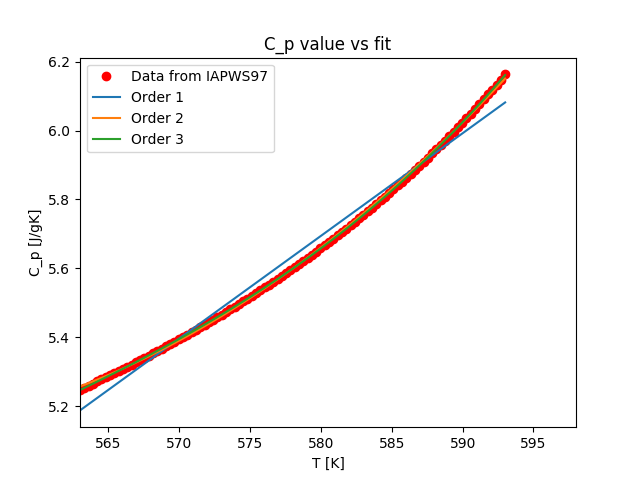
\includegraphics[scale=0.7]{cp_plot.png}
    \end{center}
    \caption{Temperature vs Heat Capacity from 563K to 598K}
    \label{fig:poly_fit}
\end{figure}


Considering the last three terms have little difference, we 
fit a second-order polynomial to obtain:

\[C_p = 4.67e-4T^2 -5.1e-1T + 144\]

Thus, using the second order polynomial fit, the volumetric
and linear heat generation becomes:

\[q'''(z) = 164.1 sin(\frac{\pi z}{L})\]
\[q'(z) = 113.8 sin(\frac{\pi z}{L})\]


\subsection*{Discuss.}
The answers to both a and b are quite similar, with minor differences.
The small difference may be due to the short temperature range where
the $C_p$ values are fitted. The little room for error is also reflected
on the almost-negligible change in the C value with change in the number of 
order fits. The volumetric heat generation with respect to height is plotted in
figure \ref{fig:q_vol}

\begin{figure}[htbp!]
    \begin{center}
        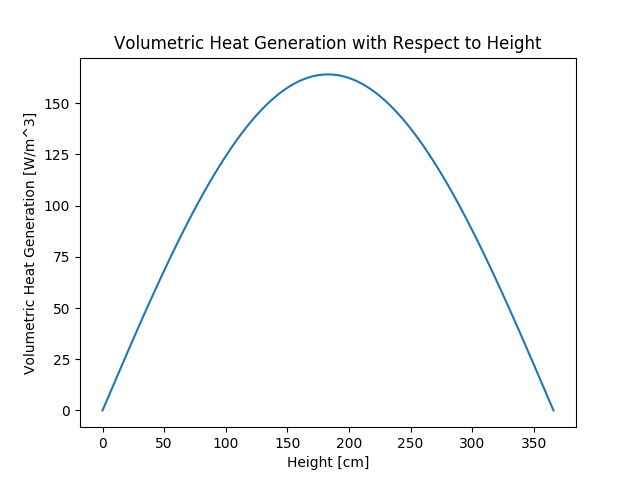
\includegraphics[scale=0.7]{q_vol_z.png}
    \end{center}
    \caption{Volumetric heat generation with respect to height obtained by polynomial fit.}
    \label{fig:q_vol}
\end{figure}




\section*{Coolant Temperature Profile}
With the heat generation found, it can be plugged back
into the energy equation to find $T_c(z)$:

\[[Area] \int^{z}_0 q'''(z) dz = \int^{T_c (z)}_{T_{in}} C_p(T) \dot{m} dT\]
\[\pi (.47^2) * 164.1 \int^{z}_0 sin(\frac{\pi z}{L})  dz =
    130.29 \int^{T_c (z)}_{T_{in}} (4.67e-4T^2 -5.1e-1T + 144)  dT\]
\[\pi (.47^2) * 164.1 * (\frac{L}{\pi} (1-cos(\frac{\pi z}{L}))) =
    130.29 (1.5e-4T^3 - .255T^2 + 144 T \Big{|}^{T_c (z)}_{T_{in}})\]

Putting numerical values instead of constants:

\[\pi (.47^2) * 164.1 * (\frac{366}{\pi} (1-cos(\frac{\pi z}{L}))) =
    130.29 (1.5e-4T^3 - .255T^2 + 144 T \Big{|}^{T_c (z)}_{563})\]

\[101.82 (1- cos(\frac{\pi z}{L})) + 27012 = 1.5e-4T_c^3 - .255T_c^2 + 144 T_c \]

\[-101.82 cos(\frac{\pi z}{L}) + 27114 = 1.5e-4T_c^3 - .255T_c^2 + 144 T_c \]

\[ cos(\frac{\pi z}{L}) = -1.47e-6T_c^3 + 0.0025T_c^2 -1.41 T_c + 265\]

To find $T_c(z)$, a root solver is used for every z value(code in appendix).
The coolant temperature profile is plotted in figure \ref{fig:t_c_z}.

\begin{figure}[htbp!]
    \begin{center}
        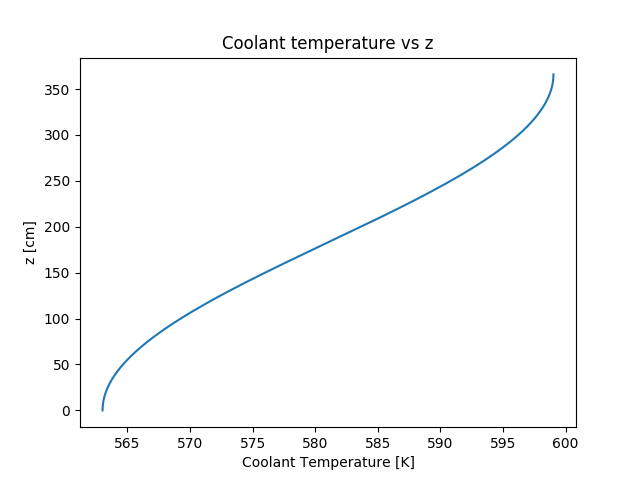
\includegraphics[scale=0.7]{t_c_z.png}
    \end{center}
    \caption{Temperature of coolant with respect to z.}
    \label{fig:t_c_z}
\end{figure}


\section*{Getting the heat transfer coefficient}
The heat transfer coefficient is obtained using the Dittus-Bolter Correlation,
where the Nusselt number is a function of the heat transfer coefficient.

\[ Nu = 0.023 Re^{0.8} Pr^{0.4} = \frac{h L}{k}\]

\[ Nu = 0.023 (\frac{\rho v L}{\mu})^{0.8} (\frac{\mu C_p}{k})^{0.4} = \frac{h L}{k}\]

where
\[v = \text{velocity of fluid} = 350 \frac{cm}{s}\]
\[L = \text{Characteristic length} = .31 cm \]
\[\rho = \text{Density of Fluid} \approx 0.7096 \frac{g}{cm^3}\]
\[\mu = \text{viscosity of fluid} \approx 0.00086 \frac{g}{cm s}\]
\[C_p = \text{ Specific Heat of fluid} \approx 5.650 \frac{J}{g K} \]
\[k = \text{thermal conductivity of fluid} \approx 0.00563\frac{W}{cm K} \]

the ones with $\approx$ are values that change with temperature. The temperature
for the approximate values are at 573K. Given this temperature, the Nusselt Number 
becomes 197.17, and heat transfer coefficient 3.5854 $\frac{W}{cm^2 K}$.

For different values of temperature given at different heights, the heat
transfer coefficient was calculated and plotted using a script (in appendix).
The plot is shown in figure \ref{fig:h_z}

\begin{figure}[htbp!]
    \begin{center}
        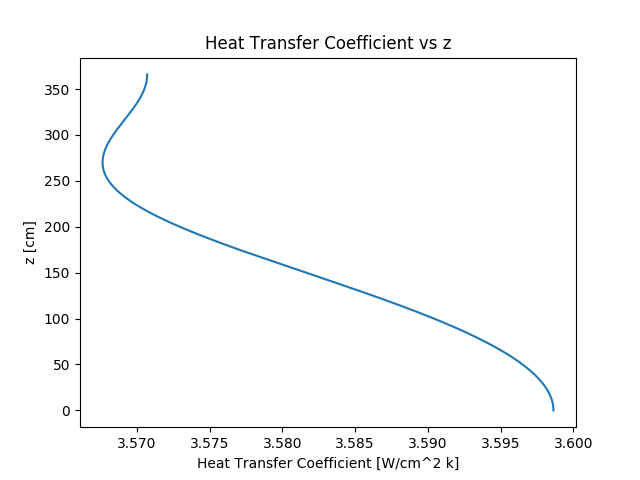
\includegraphics[scale=0.7]{h_z.png}
    \end{center}
    \caption{Heat Transfer Coefficient vs Z.}
    \label{fig:h_z}
\end{figure}

\section*{Using Computer Code for Temperature Distribution in Fuel Rod}

The temperature in the fuel rod is governed by the differential equation:
\[ \frac{d^2T}{dz^2} + \frac{1}{r} \frac{d}{dr} (r \frac{dT}{dr}) + \frac{q'''(z)}{k} = 0\]

\[ \frac{d^2T}{dz^2} + (\frac{d^2T}{dr^2} + \frac{1}{r} \frac{dT}{dr}) + \frac{q'''(z)}{k} = 0\]

Using the finite difference method, the differential equation becomes,

\[\frac{u_{z+1}^r - 2u_z^r + u_{z-1}}{dz^2}^r + \frac{u^{r+1}_z - 2u^r_z + u^{r-1}_z}{dr^2}
  + \frac{1}{r} \frac{u^{r+1}_z - u^{r-1}_z}{2dr} + \frac{q_z^r}{k} = 0 \]

solving for $u_z^r$:

\[ u_z^r = \frac{\frac{u_{z+1}^r + u_{z-1}^r}{dz^2} + \frac{u^{r+1}_z + u^{r-1}_z}{dr^2}
  + \frac{1}{r} \frac{u^{r+1}_z - u^{r-1}_z}{2dr} + \frac{q_z}{k}}{\frac{2}{dz^2} + \frac{2}{dr^2}} \]

With boundary conditions:

\begin{enumerate}
    \item $\frac{dT}{dr}(r=0) = 0$
    \item $-k \frac{dT}{dr} (r=R) = h(T(r=R) - T_c)$
    \item $\frac{dT}{dz}(z=0) = 0 $
    \item $\frac{dT}{dz}(z=L) = 0 $
\end{enumerate}

using finite difference, the boundary conditions become the following.
The first index is the z element, and the second the r element. The indexing
standard follows Python.
\begin{enumerate}
    \item $u[z][1]-u[z][0] = 0$
    \item $-k \frac{u[z][-2]-u[z][-1]}{dr} = h(u[z][-1] - T_c)$
    \item $ \frac{u[1][r] - u[0][r]}{dz} = 0$
    \item $\frac{u[-2][r] - u[-1][r]}{dz} = 0 $
\end{enumerate}




\section*{Analytically Solve 1D Fuel Temperature Profile}
Ignoring Axial Conduction, we get:

\[\frac{1}{r} \frac{d}{dr} (r \frac{d^T}{dr}) = \frac{-q'''(z)}{k}\]
\[k = 0.057 \frac{W}{cm\cdot K}\]

q'''(z) and $T_c$, and h  values for z values L/4, L/2, 3L/4 are listed in table \ref{tab:q_vol}.
The values are obtained from previous problems, and using a script (in appendix).
The value of thermal conductivity of uranium oxide is assumed
to be 0.4.\cite{ronchi_thermal_1999}.

\begin{table}[h]
     \centering
    \begin{tabular}{cccc}
       \hline
       z value & q'''(z) [W/cmK] & $T_c(z) [K]$ & $h [\frac{W}{cm^2 K}] $ \\
       \hline
       L/4 & 116.03 & 568.2 & 3.591 \\
       L/2 & 164.1 & 581.04 & 3.575 \\
       3L/4 & 116.03 & 593.78 & 3.567 \\
       \hline
    \end{tabular}
    \caption {q'''(z), $T_c$ and h value for various z values}
    \label{tab:q_vol}
\end{table}

Integrating the differential equation to obtain the temperature profile for the
1D fuel:


\[ (r \frac{dT}{dr}) = \frac{-q'''(z)r^2}{2k} + C_1 \]

\[ \frac{dT}{dr} = \frac{-q'''(z)r}{2k} + \frac{C_1}{r} \]

\[ T_{1D} = \frac{-q'''(z)r^2}{4k} + C_1 ln(r) + C_2 \]
Applying BC at r=0, $C_1$ = 0.
Applying convective BC:
\[ -k \frac{dT}{dr}(r= 0.47 cm) = h (T(r = 0.47 cm ) - T_{coolant})\]
\[ k( \frac{q'''R}{2k}) = h (\frac{-q'''R^2}{4k} + C_2 + T_{coolant})\]
This makes:
\[C_2 = \frac{q'''R}{2} + \frac{hq'''R^2}{4k} + hT_{coolant}\]

\[ T_{1D} = \frac{-q'''(z)r^2}{4k} + \frac{q'''(z)R}{2} + \frac{hq'''R^2}{4k} + hT_{coolant}\]


The $C_2$ values obtained with the equation is listed in table \ref{tab:c2}.
The fuel temperature is plotted in figure \ref{fig:t_f_r}.

\begin{table}[h]
     \centering
    \begin{tabular}{ccc}
       \hline
       z value & $C_2$ & equation \\
       \hline
       L/4 & 323.6  & $T_{1D} = -\frac{-q'''(z)r^2}{4k} + 323.6$ \\
       L/2 & 234.29 & $T_{1D} = -\frac{-q'''(z)r^2}{4k} + 234.29$ \\
       3L/4 & 348.30 & $T_{1D} = -\frac{-q'''(z)r^2}{4k} + 348.3$\\
       \hline
    \end{tabular}
    \caption {$C_2$ value for different z values}
    \label{tab:c2}
\end{table}


\begin{figure}[htbp!]
    \begin{center}
        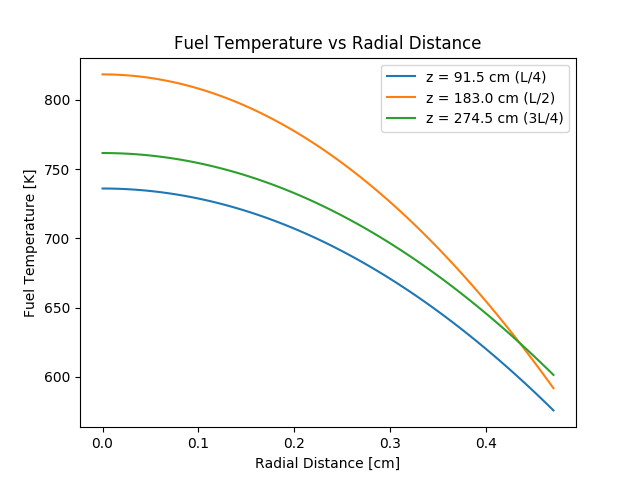
\includegraphics[scale=0.7]{t_f_r.png}
    \end{center}
    \caption{Temperature of Fuel with respect to r for different z values.}
    \label{fig:t_f_r}
\end{figure}

\section*{Varying Density with temperature}
Since temperature in the coolant varies with height in the core,
the density changes as well. The same module used to obtain $C_p$
is used to obtain the density values \cite{romera_iapws:_2017}.
Plugging in the temperature value to obtain the density value, we get
figure \ref{fig:rho_c_z}

\begin{figure}[htbp!]
    \begin{center}
        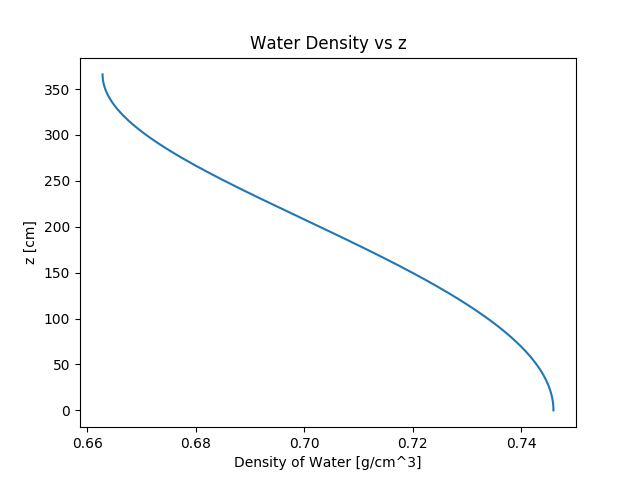
\includegraphics[scale=0.7]{rho_c_z.png}
    \end{center}
    \caption{Density of Coolant with respect to z.}
    \label{fig:rho_c_z}
\end{figure}



\pagebreak
Differential Equation:

For water channel ($R_i \leq r \leq R_o$):
\[\frac{1}{\alpha} \cdot (\frac{dT}{dt} + (V_r \frac{dT}{dr} + V_z \frac{dT}{dz})) =
  \frac{1}{dr} \frac{d}{dr} (r \frac{dT}{dr}) + \frac{d^2T}{dz^2})\]

For fuel pin ($r < R_i$):
\[\frac{1}{\alpha} \cdot (\frac{dT}{dt}) =
  \frac{1}{dr} \frac{d}{dr} (r \frac{dT}{dr}) + \frac{d^2T}{dz^2}) + \frac{q(z)}{k}\]

Boundary Conditions:
\[-k \frac{dT}{dr}(z=R_o) = 0 \]
\[\frac{dT}{dr}(r=0) = 0\]
\[-k \frac{dT}{dz}(z=0) = -k \frac{dT}{dz}(z=L) = 0 \]
 

Initial Condition:
\[T(r,0) = \frac{T_0}{2} (1-\cos{(\frac{\pi \cdot r}{R})}) \]




\bibliographystyle{abbrv}
\bibliography{bibliography}
\pagebreak


\begin{appendices}

\section{For fitting polynomials for Heat Capacity}

\begin{minted}{python}
def fit_poly_cp(order):
    """ fits a polynomial for Temp and C_p of Water"""
    temp = np.linspace(290+273, 320+273, 100)
    cp =[]
    for i in temp:
        cp.append(IAPWS97(T=i, P=15.17).cp)
    eq = np.polyfit(temp, cp, order)
    eq = list(reversed(eq))
    x =np.polynomial.polynomial.Polynomial(eq)
    integral = integrate.quad(x, 290+273, 325+273)
    print('Result of the Integral for order %s is:' %str(order))
    print(integral[0])
    print('C = ')
    print(132.446*integral[0] / (366*2*.47**2))
    print('\n \n')
\end{minted}

\section{For finding $T_c(z)$}

\begin{minted}{python}
def root_solver():
    """ fits a polynomial for Temp and C_p of Water"""
    z = np.linspace(0, 366, 100)
    t_c = []
    for i in z:
        root = np.roots([-1.47e-6, 0.0025, -1.41, 276.23-np.cos(np.pi * i / 366)])
        print(root)
        print(type(root))
        filtered_root = float(str(root[0])[1:7])
        t_c.append(filtered_root)

    plt.plot(t_c, z)
    plt.show()
\end{minted}

\section{For finding h}

\begin{minted}{python}

def find_h():
    ri = 0.47
    ro = 0.625
    v = 350
    for i in [568.2, 581.04, 593.78]:
        L = 4 * np.pi*(ro**2 - ri**2) / (2*np.pi*ro + 2*np.pi*ri)
        mu = IAPWS97(T=i, P=15.17).mu * 10
        rho = IAPWS97(T=i, P=15.17).rho /1000
        cp = IAPWS97(T=i, P=15.17).cp
        k = IAPWS97(T=i, P=15.17).k /100
        Re = rho*v*L / mu
        Pr = mu*cp / k
        Nu = 0.023 * Re**(0.8) * Pr**(0.4)
        h = Nu * k / L
        print(h)
        print('\n')
\end{minted}


\end{appendices}
\pagebreak

-end of report.
\end{document}






